\section{Results}
\begin{figure*}[!t]\centering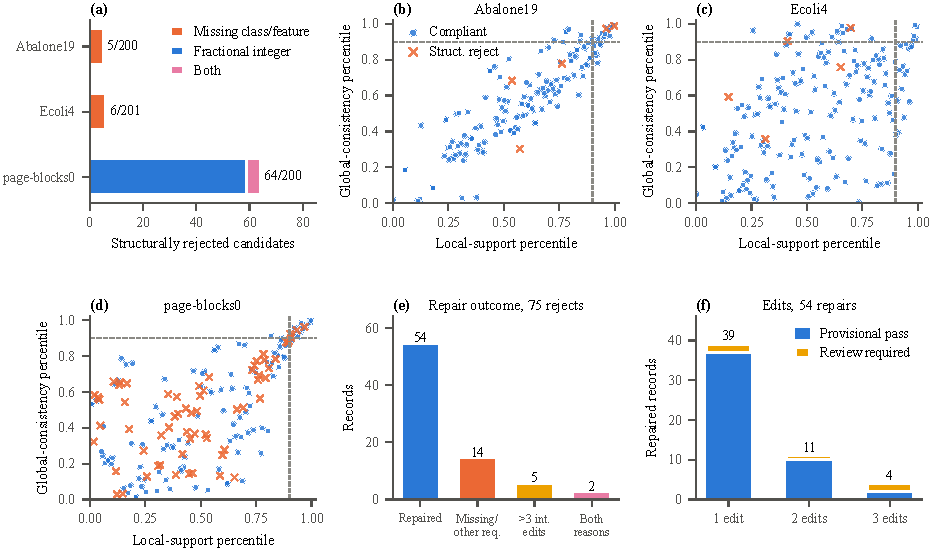
\includegraphics[width=\textwidth]{figures/audit.pdf}
\caption{Historical candidate audit. (a) Structural rejects by violation type. (b--d) Local-support and global-consistency percentiles of every candidate with available evidence; dashed lines mark the review cutoff $q=.90$, crosses mark structural rejects. (e) Repair outcome for the 75 rejects. (f) Integer edits per repaired record and admission after rescoring.}\label{fig:audit}\end{figure*}

\subsection{RQ1--RQ2: structure and complementary support}
There are 75 structural rejects (12.48\%): five of 200 Abalone19, six of 201 Ecoli4 and 64 of 200 page-blocks0 candidates (Fig.~\ref{fig:audit}a). Fifteen lack class, one lacks features and 64 have fractional-integer fields; 26 violate multiple fields, and no unsupported nominal value or invalid numerical primitive appears. Local and global evidence are related but flag different records (Fig.~\ref{fig:audit}b--d): Spearman correlations are $.908$, $.488$ and $.621$ for Abalone19, Ecoli4 and page-blocks0, with 14, 30 and two tail disagreements. Combined admission yields 170, 162 and 119 provisional passes, against 195, 195 and 136 with structure only. This shows distinct statistical information, not semantic-error detection performance.

\subsection{RQ3: matched-budget ablations}
\begin{table*}[!t]
\centering
\caption{Consolidated historical ablations. Q denotes unchanged quality-coverage selection. Random rows average five seeds; complete per-seed data accompany the paper. F1 is logistic pure TSTR; -- means unavailable.}\label{tab:ablations}
\footnotesize\setlength{\tabcolsep}{6pt}
\begin{tabular}{lrrrrrrr}
\toprule
Dataset & Method & Pool & $n$ & Coverage & Exact & Near & F1 \\
\midrule
Abalone19 & Raw labeled random & 195 & 56 & 0.799 & 0.171 & 0.443 & 0.029 \\
 & Schema random & 195 & 56 & 0.799 & 0.171 & 0.443 & 0.029 \\
 & Admitted random & 170 & 56 & 0.833 & 0.236 & 0.493 & 0.022 \\
 & Structure + Q selection & 195 & 56 & 0.951 & 0.000 & 0.000 & 0.030 \\
 & Structure/local + Q & 177 & 56 & 0.950 & 0.000 & 0.000 & 0.031 \\
 & Structure/global + Q & 177 & 56 & 0.948 & 0.000 & 0.000 & 0.031 \\
 & Structure/local/global + Q & 170 & 56 & 0.948 & 0.000 & 0.000 & 0.031 \\
 & Admitted source order & 170 & 56 & 0.622 & 0.357 & 0.625 & -- \\
 & Admitted farthest first & 170 & 56 & 0.940 & 0.000 & 0.000 & 0.035 \\
 & Admitted coverage greedy & 170 & 56 & 0.948 & 0.107 & 0.268 & 0.030 \\
 & Repair pool + Q & 170 & 56 & 0.948 & 0.000 & 0.000 & 0.031 \\
Ecoli4 & Raw labeled random & 195 & 70 & 0.422 & 0.097 & 0.180 & 0.253 \\
 & Schema random & 195 & 70 & 0.422 & 0.097 & 0.180 & 0.253 \\
 & Admitted random & 162 & 70 & 0.439 & 0.117 & 0.197 & 0.217 \\
 & Structure + Q selection & 195 & 70 & 0.509 & 0.000 & 0.000 & 0.216 \\
 & Structure/local + Q & 175 & 70 & 0.509 & 0.000 & 0.000 & 0.195 \\
 & Structure/global + Q & 177 & 70 & 0.506 & 0.000 & 0.000 & 0.229 \\
 & Structure/local/global + Q & 162 & 70 & 0.506 & 0.000 & 0.000 & 0.205 \\
 & Admitted source order & 162 & 70 & 0.416 & 0.200 & 0.386 & -- \\
 & Admitted farthest first & 162 & 70 & 0.468 & 0.000 & 0.000 & 0.200 \\
 & Admitted coverage greedy & 162 & 70 & 0.506 & 0.114 & 0.243 & 0.108 \\
 & Repair pool + Q & 162 & 70 & 0.506 & 0.000 & 0.000 & 0.205 \\
page-blocks0 & Raw labeled random & 195 & 49 & 0.905 & 0.061 & 0.559 & 0.390 \\
 & Schema random & 136 & 49 & 0.889 & 0.069 & 0.559 & 0.477 \\
 & Admitted random & 119 & 49 & 0.914 & 0.082 & 0.702 & 0.535 \\
 & Structure + Q selection & 136 & 49 & 0.934 & 0.000 & 0.286 & 0.202 \\
 & Structure/local + Q & 120 & 49 & 0.932 & 0.000 & 0.327 & 0.446 \\
 & Structure/global + Q & 120 & 49 & 0.934 & 0.000 & 0.327 & 0.448 \\
 & Structure/local/global + Q & 119 & 49 & 0.932 & 0.000 & 0.327 & 0.446 \\
 & Admitted source order & 119 & 49 & 0.914 & 0.265 & 0.592 & -- \\
 & Admitted farthest first & 119 & 49 & 0.932 & 0.000 & 0.000 & 0.550 \\
 & Admitted coverage greedy & 119 & 49 & 0.932 & 0.163 & 0.449 & 0.627 \\
 & Repair pool + Q & 168 & 49 & 0.937 & 0.000 & 0.102 & 0.342 \\
\bottomrule
\end{tabular}
\end{table*}

\begin{figure*}[!t]\centering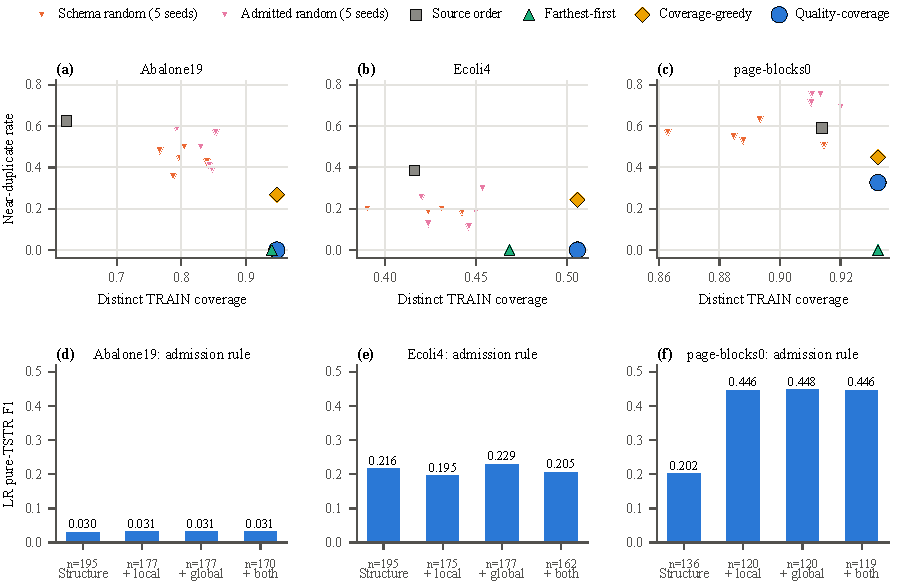
\includegraphics[width=\textwidth]{figures/construction.pdf}
\caption{Historical matched-budget construction. (a--c) Distinct-feature TRAIN coverage against near-duplicate rate; random controls show all five seeds, and deterministic selectors share the admitted pool (on Abalone19, farthest-first and quality-coverage nearly coincide). (d--f) Logistic pure-TSTR F1 after quality-coverage selection under each admission rule; $n$ is the eligible pool.}\label{fig:construction}\end{figure*}
Every construction reaches its budget (Table~\ref{tab:ablations}, Fig.~\ref{fig:construction}). Quality-coverage raises distinct-feature TRAIN coverage over source order from $.6225$ to $.9479$ on Abalone19 and from $.4164$ to $.5056$ on Ecoli4, with zero exact and near redundancy. Farthest-first also removes redundancy but covers less of Ecoli4 ($.4684$); coverage-greedy matches $.5056$ with exact duplication $.1143$. Eligibility, quotas and coverage act together, so this is not the isolated effect of an evidence score. Additional evidence also changes outcomes non-monotonically: structure-only admission slightly exceeds full-admission coverage on Abalone19 ($.951$ versus $.948$) and Ecoli4 ($.509$ versus $.506$), whereas on page-blocks0 full admission raises logistic pure-TSTR F1 from $.202$ to $.446$.

\subsection{RQ4: bounded repair}
All 54 eligible repairs become compliant; 21 rejects are ineligible (Fig.~\ref{fig:audit}e), including five page-blocks0 records that also lack class and five that need more than three edits. Repairs edit 73 fields: 39 records need one edit, eleven two and four three, with absolute changes of $.1$--$.5$ (mean $.3119$). Under unchanged admission, 49 repaired versions provisionally pass and five need review, so the page-blocks0 admitted pool grows from 119 to 168. At budget 49, quality-coverage selects 16 repaired records: coverage rises from $.9324$ to $.9370$ and near duplication falls from $.3265$ to $.1020$. Source-order coverage declines slightly, so expanded pools have method-dependent effects.

\subsection{RQ5: utility and external comparators}
All 138 historical utility rows reproduce within $10^{-12}$. The expanded study has 894 utility rows, 678 successful and 216 explicitly unavailable, with no execution failures or budget shortfalls.
\begin{table*}[!t]
\centering
\caption{Historical external training baselines. ROS and SMOTE/NC append b minority rows. LR: logistic regression; RF: random forest. These differ from candidate curation.}\label{tab:external}
\footnotesize\setlength{\tabcolsep}{6pt}
\begin{tabular}{lrrrrrr}
\toprule
Dataset / method & Model & $+n$ & F1 & AP & BA & MCC \\
\midrule
Abalone19 / Real & LR & 0 & 0.000 & 0.026 & 0.500 & 0.000 \\
Abalone19 / Real & RF & 0 & 0.000 & 0.023 & 0.500 & 0.000 \\
Abalone19 / Weighted LR & LR & 0 & 0.054 & 0.038 & 0.873 & 0.144 \\
Abalone19 / ROS+b & LR & 56 & 0.000 & 0.031 & 0.500 & 0.000 \\
Abalone19 / ROS+b & RF & 56 & 0.000 & 0.031 & 0.500 & 0.000 \\
Abalone19 / SMOTENC+b & LR & 56 & 0.000 & 0.014 & 0.499 & -0.003 \\
Abalone19 / SMOTENC+b & RF & 56 & 0.000 & 0.020 & 0.499 & -0.003 \\
Ecoli4 / Real & LR & 0 & 1.000 & 1.000 & 1.000 & 1.000 \\
Ecoli4 / Real & RF & 0 & 0.667 & 1.000 & 0.750 & 0.696 \\
Ecoli4 / Weighted LR & LR & 0 & 0.800 & 1.000 & 0.984 & 0.803 \\
Ecoli4 / ROS+b & LR & 70 & 1.000 & 1.000 & 1.000 & 1.000 \\
Ecoli4 / ROS+b & RF & 70 & 0.857 & 1.000 & 0.875 & 0.859 \\
Ecoli4 / SMOTE+b & LR & 70 & 1.000 & 1.000 & 1.000 & 1.000 \\
Ecoli4 / SMOTE+b & RF & 70 & 0.857 & 1.000 & 0.875 & 0.859 \\
page-blocks0 / Real & LR & 0 & 0.715 & 0.746 & 0.802 & 0.699 \\
page-blocks0 / Real & RF & 0 & 0.869 & 0.921 & 0.911 & 0.856 \\
page-blocks0 / Weighted LR & LR & 0 & 0.721 & 0.768 & 0.903 & 0.696 \\
page-blocks0 / ROS+b & LR & 49 & 0.728 & 0.746 & 0.811 & 0.712 \\
page-blocks0 / ROS+b & RF & 49 & 0.864 & 0.920 & 0.906 & 0.851 \\
page-blocks0 / SMOTE+b & LR & 49 & 0.728 & 0.758 & 0.811 & 0.712 \\
page-blocks0 / SMOTE+b & RF & 49 & 0.869 & 0.916 & 0.911 & 0.856 \\
\bottomrule
\end{tabular}
\end{table*}

The external baselines (Table~\ref{tab:external}) are training alternatives, not matched curation. Standard SMOTE output for page-blocks0 is not integer-coerced, so 46 of 49 generated rows fail the integer contract while remaining evaluable numerical augmentation.

Geometry and utility can disagree. For page-blocks0 logistic pure TSTR, repair-pool expansion lowers F1 from $.4464$ to $.3421$, while AP moves from $.5552$ to $.5716$ and hybrid F1 stays $.7150$, despite the coverage and redundancy gains of RQ4.

\subsection{RQ6: conditional uncertainty and fresh-split stability}
\begin{figure*}[!t]\centering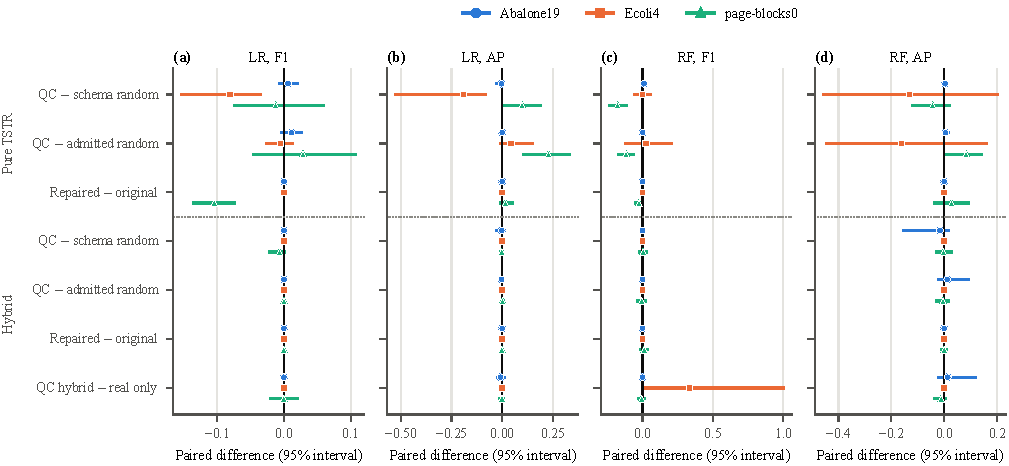
\includegraphics[width=\textwidth]{figures/uncertainty.pdf}
\caption{Conditional paired 95\% intervals for the primary historical pairs (2,000 stratified resamples of saved predictions); markers are observed differences. Intervals condition on the fitted models and the reused historical TEST set; endpoint intervals are in Appendix Table~\ref{tab:bootstrap}.}\label{fig:uncertainty}\end{figure*}
Saved predictions give 216 endpoint and 168 paired-difference intervals (Fig.~\ref{fig:uncertainty}). The page-blocks0 logistic repair-minus-original F1 difference is about $-.1043$ (interval $[-.1350,-.0739]$) and the AP difference $.0165$ ($[-.0071,.0493]$): F1 decreases consistently under this design, while the AP direction is less stable. Small positive counts limit the rest. Ecoli4 logistic TRTR predicts its four positive and 63 negative TEST records perfectly, giving F1 interval $[1,1]$ but a Wilson positive-recall interval of about $[.510,1]$, and Abalone19 has six TEST positives; resampling adds no independent positive observations.

\begin{figure*}[!t]\centering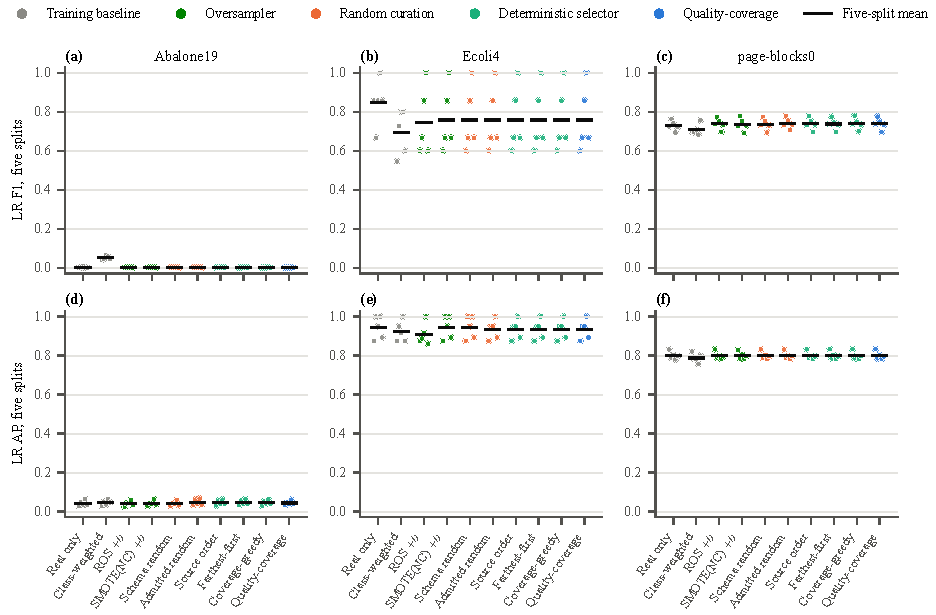
\includegraphics[width=\textwidth]{figures/fresh-splits.pdf}
\caption{Offline replication on five fresh stratified splits: logistic F1 (a--c) and AP (d--f) per split with five-split means. Curators use the hybrid regime; real-only and class-weighted training use TRTR; the page-blocks0 pool generator is ROS. Summary statistics are in Appendix Table~\ref{tab:repeated}.}\label{fig:fresh}\end{figure*}
All 15 split-specific runs complete (Fig.~\ref{fig:fresh}). Ecoli4 logistic F1 is $.8476\pm.1186$ for real-only training and $.7581\pm.1659$ for quality-curated augmentation, the same mean as admitted random. Abalone19 F1 stays zero under real-only training and every augmentation method, while balanced logistic loss reaches $.0506\pm.0095$. On page-blocks0, real-only F1 is $.7284\pm.0256$, quality-curated augmentation $.7383\pm.0283$ and admitted random $.7409\pm.0270$. Augmentation brings no uniform benefit and does not beat simple curation.
